\part{Evolutionary algorithms}
\frame{\partpage}

\begin{frame}{Evolutionary algorithms (EAs)}
	\begin{itemize}
		\pause\item Optimisation technique inspired by \textbf{biological evolution}
		\pause\item We have a \textbf{population} of $N$ solutions
		\pause\item Generation $0$: choose $N$ solutions at random
		\pause\item Generation $i+1$: choose $N$ new solutions based on the \textbf{fittest} individuals from generation $i$
	\end{itemize}
\end{frame}

\begin{frame}{Selecting the fittest}
	\begin{itemize}
		\pause\item \textbf{All} individuals should have a \textbf{chance} of being selected
		\pause\item But \textbf{fitter} individuals should be selected \textbf{more often}
		\pause\item Simple method: \textbf{tournament selection}
			\begin{itemize}
				\pause\item Randomly choose $t$ individuals
				\pause\item Select the fittest out of those $t$
			\end{itemize}
	\end{itemize}
\end{frame}

\begin{frame}{Mutation}
	\begin{itemize}
		\pause\item Select an individual
		\pause\item Make a small change to it
		\pause\item Add the changed individual to the new population
	\end{itemize}
\end{frame}

\begin{frame}{Crossover}
	\begin{itemize}
		\pause\item Select two individuals
		\pause\item Combine them somehow (take ``half'' of one and ``half'' of the other)
		\pause\item Add the resulting individual to the new population
	\end{itemize}
\end{frame}

\begin{frame}{Elitism}
	\begin{itemize}
		\pause\item Take the top $x\%$ of generation $i$, and pass it straight through to generation $i+1$
	\end{itemize}
\end{frame}

\begin{frame}{Not just for PCG}
	\begin{itemize}
		\pause\item Common use for optimisation: \textbf{parameter tuning}
		\pause\item Suppose we have several simple heuristic evaluation functions (or utility functions) $h_1, h_2, \dots, h_n$
			which we want to combine into a single heuristic
		\pause\item \textbf{Linear combination}:
			$$ w_1 h_1 + w_2 h_2 + \dots + w_n h_n $$
			where $w_1, w_2, \dots, w_n$ are constants: \textbf{weights}
		\pause\item What value to choose for the weights? This is an optimisation problem!
	\end{itemize}
\end{frame}

\begin{frame}{Genetic programming}
    \begin{columns}
        \begin{column}{0.48\textwidth}
            \pause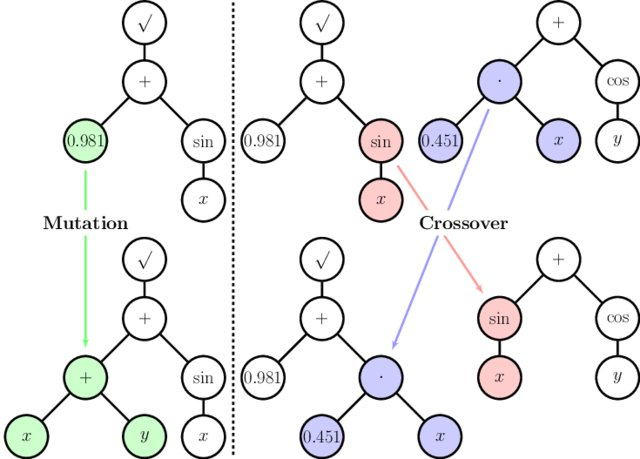
\includegraphics[width=\textwidth]{genetic_programming}
        \end{column}
        \begin{column}{0.48\textwidth}
            \begin{itemize}
                \pause\item Evolutionary algorithms for generating \textbf{code}
                \pause\item Typically uses a \textbf{tree-based} representation of code
                \pause\item Other approaches exist e.g.\ template-based
            \end{itemize}
        \end{column}
    \end{columns}
\end{frame}
